\begin{frame}{Task 3: Idea to a literature review, report, or proposal}
  \ndlogonote{\scriptsize\href{https://github.com/dowlinglab/claude-for-researchers/blob/main/resources/practices/technical_writing.md}{\texttt{resources/practices/technical\_writing.md}}}
  \vfill
  \begin{columns}[t]
    \begin{column}{0.46\textwidth}
      \textbf{What is \LaTeX?}
      \begin{itemize}\small\setlength\itemsep{0.4em}
        \item a plain-text document source
        \item separates content from layout
        \item compiles to a PDF
        \item built for equations, references, and cross-references
      \end{itemize}
    \end{column}
    \begin{column}{0.48\textwidth}
      \textbf{Why agents work well with it}
      \begin{itemize}\small\setlength\itemsep{0.4em}
        \item the source is searchable text
        \item sections and figures are separate files
        \item every edit produces a readable diff
        \item the compiled PDF is a visual check
      \end{itemize}
    \end{column}
  \end{columns}
  \vspace{1.0em}
  \begin{center}
    \slidepoint{Plain text is what lets an agent --- and Git --- work on your manuscript.}
  \end{center}
  \vspace{1.1cm plus 1fill}
\end{frame}

\begin{frame}{Overleaf and local edits meet through GitHub}
  \ndlogonote{\scriptsize\href{https://docs.overleaf.com/integrations-and-add-ons/git-integration-and-github-synchronization/github-synchronization}{Overleaf: GitHub synchronization (documentation + screenshot)}\quad\href{https://github.com/dowlinglab/claude-for-researchers/blob/main/resources/practices/latex_overleaf_workflow.md}{Companion workflow}}
  \vfill
  \begin{columns}[c]
    \begin{column}{0.46\textwidth}
      \centering
      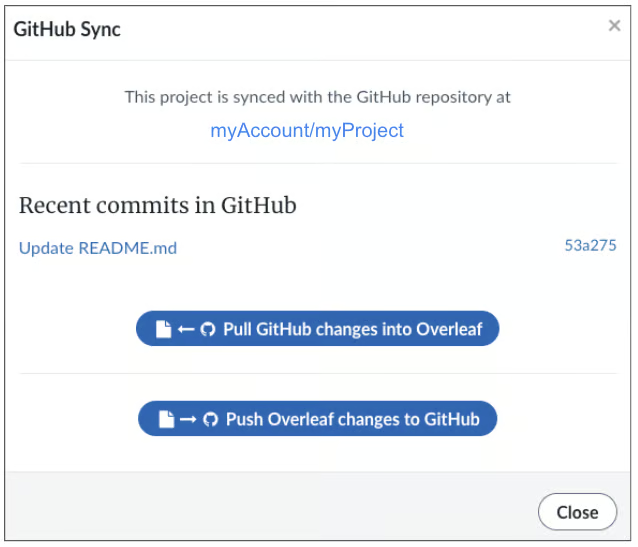
\includegraphics[width=\linewidth,height=4.9cm,keepaspectratio]{figures/overleaf_github_sync.png}
    \end{column}
    \begin{column}{0.49\textwidth}
      \begin{enumerate}\small\setlength\itemsep{0.7em}
        \item Sync Overleaf edits to GitHub; pull locally.
        \item Revise on a \textbf{feature branch}.
        \item Incorporate collaborators' latest changes; review and merge.
        \item Pull the merged version into Overleaf.
      \end{enumerate}
      \vspace{0.5em}
      \small Synchronization is \textbf{explicit}, not automatic. Coordinate with coauthors.
    \end{column}
  \end{columns}
  \vspace{0.8cm plus 1fill}
\end{frame}

\begin{frame}{Three repositories keep development, writing, and release separate}
  \ndlogonote{\scriptsize\href{https://github.com/dowlinglab/claude-for-researchers/blob/main/resources/practices/latex_overleaf_workflow.md}{\texttt{resources/practices/latex\_overleaf\_workflow.md}}}
  \vfill
  \begin{center}\small
  \renewcommand{\arraystretch}{1.22}
  \begin{tabular}{@{}>{\raggedright\arraybackslash}p{3.1cm}>{\raggedright\arraybackslash}p{5.1cm}>{\raggedright\arraybackslash}p{4.3cm}@{}}
    \toprule
    \textbf{Repository} & \textbf{What belongs there} & \textbf{History} \\
    \midrule
    Private code & data, experiments, analysis & rich history; my projects: 10--500 MB \\
    Private writing & \LaTeX{}, bibliography, selected figures & compact history; sync recommendation: $<100$ MB \\
    Public release & package and paper reproduction & near-final history for readers \\
    \bottomrule
  \end{tabular}
  \end{center}
  \vspace{0.7em}
  \begin{itemize}\small\setlength\itemsep{0.4em}
    \item Keep individual Git files below about \textbf{10 MB}.
    \item Put large PDF collections on a shared drive, not in Git.
    \item Keep the summaries and \texttt{ref.bib} in Git.
  \end{itemize}
  \vspace{1.0cm plus 1fill}
\end{frame}

\begin{frame}{Task 3, step 1: Search, read, and search again}
  \ndlogonote{\scriptsize\href{https://github.com/dowlinglab/claude-for-researchers/blob/main/resources/practices/literature_review.md}{\texttt{resources/practices/literature\_review.md}}}
  \vfill
  \begin{enumerate}\setlength\itemsep{0.8em}
    \item \textbf{Frame the question with a chatbot}
      \begin{itemize}\small
        \item develop terminology, synonyms, and adjacent disciplines
        \item turn the idea into several targeted search strings
      \end{itemize}
    \item \textbf{Search Google Scholar and disciplinary databases}
      \begin{itemize}\small
        \item follow review papers, citation trails, and competing terminology
        \item download only papers you can identify and inspect
      \end{itemize}
    \item \textbf{Repeat after each processed batch}
      \begin{itemize}\small
        \item ask the agent which gaps, authors, and references should drive the next search
      \end{itemize}
  \end{enumerate}
  \vspace{1.0cm plus 1fill}
\end{frame}

\begin{frame}{Task 3, step 2: Build a literature corpus an agent can use}
  \ndlogonote{\scriptsize\href{https://github.com/dowlinglab/claude-for-researchers/blob/main/resources/prompts/literature_workflow.md}{\texttt{resources/prompts/literature\_workflow.md}}}
  \vfill
  \begin{enumerate}\setlength\itemsep{0.8em}
    \item \textbf{Process the PDFs in small topical batches}
      \begin{itemize}\small
        \item checkpoint after each batch
        \item propose consistent filenames; flag likely duplicates without deleting
      \end{itemize}
    \item \textbf{Maintain \texttt{ref.bib} as you go}
      \begin{itemize}\small
        \item verified metadata and DOI information, one entry per paper
      \end{itemize}
    \item \textbf{Summarize every paper in \texttt{literature.md}}
      \begin{itemize}\small
        \item contribution, evidence, relevance, and what it cannot support
        \item keep the PDFs in a reference manager; keep the text artifacts in Git
      \end{itemize}
  \end{enumerate}
  \vspace{0.6em}
  \begin{center}
    \slidepoint{The durable product is the \textbf{verified map of the literature}.}
  \end{center}
  \vspace{0.6cm plus 1fill}
\end{frame}

\begin{frame}{Task 3, step 3: Edit the document against the curated corpus}
  \ndlogonote{\scriptsize\href{https://github.com/dowlinglab/claude-for-researchers/blob/main/resources/practices/grant_proposal_writing.md}{\texttt{resources/practices/grant\_proposal\_writing.md}}}
  \vfill
  \begin{enumerate}\setlength\itemsep{0.8em}
    \item \textbf{Start from the question and \texttt{literature.md}}
      \begin{itemize}\small
        \item build a claim-and-evidence outline before writing prose
      \end{itemize}
    \item \textbf{Draft one section at a time}
      \begin{itemize}\small
        \item ask what evidence supports each paragraph before polishing it
        \item preserve uncertainty and conflicting evidence as part of the argument
      \end{itemize}
    \item \textbf{Check every claim against the source PDFs}
      \begin{itemize}\small
        \item edit against the local corpus, not an agent's memory
      \end{itemize}
  \end{enumerate}
  \vspace{1.0cm plus 1fill}
\end{frame}

\begin{frame}{Review the source diff and the manuscript diff}
  \ndlogonote{\scriptsize\href{https://github.com/dowlinglab/claude-for-researchers/tree/main/resources/examples/manuscript_revision}{Reproduce the example}\quad\href{https://docs.github.com/en/desktop/making-changes-in-a-branch/committing-and-reviewing-changes-to-your-project-in-github-desktop}{Screenshot: GitHub Docs}}
  \vfill
  \begin{columns}[c]
    \begin{column}{0.48\textwidth}
      \centering\small\textbf{GitHub Desktop: file changes}\\[0.5em]
      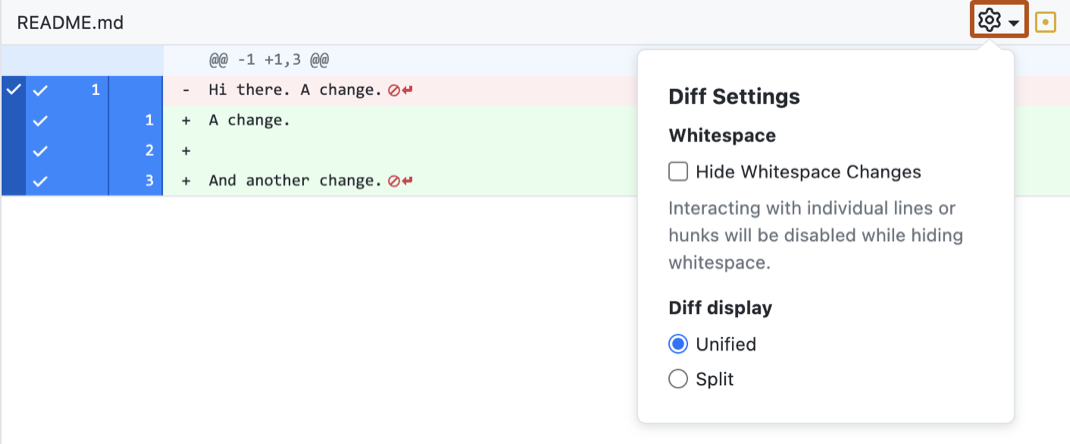
\includegraphics[width=\linewidth]{figures/github_desktop_diff.png}
    \end{column}
    \begin{column}{0.48\textwidth}
      \centering\small\textbf{\texttt{latexdiff}: manuscript changes}\\[0.5em]
      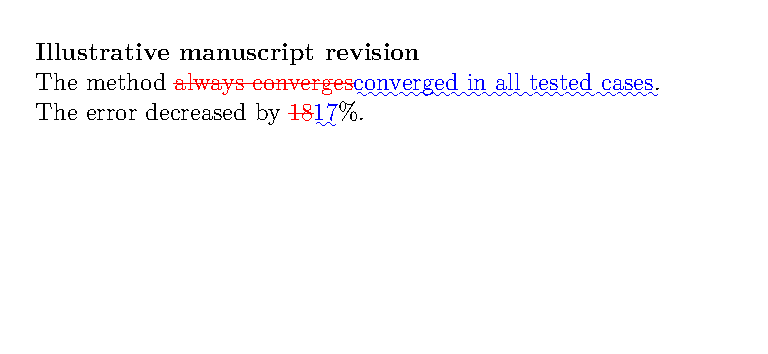
\includegraphics[width=\linewidth]{figures/manuscript_diff.pdf}
    \end{column}
  \end{columns}
  \vspace{0.8em}
  \begin{center}\small
    Ask the agent to generate and compile \texttt{latexdiff}.\\[0.35em]
    \textbf{You review the changed claims} before merging and syncing.
  \end{center}
  \vspace{0.8cm plus 1fill}
\end{frame}
